\chapter{Correlation Power Analysis} \label{c8_fifthcapter}

this lecture is the last technical lecture of the course about High Data
Complexity Power Analysis, CPA.

\section{Previous lectures recap}\label{c8_prev_lectures_recap:sec}

We are interested in laying a side-channel attack. We have a device performing
a secret operation, AES operation. The device works as follows: we give input to
the device (plain text), and then it works on the input to produce an output
(ciphertext) using a secret key. We want to recover the key. So, if we collect
many pairs of plain text and ciphertext, what can we do with that? Lots of
things. In addition to plain text and ciphertext, we have a side channel \cite{SideChannel}. What
is a side-channel? A side-channel is an artifact of the computation, and what is
careful about the channel is that it depends on the intermediate values of the
computation and not its output. We talked about the multiple side channels
throughout the course.

\subsection{Timing side channel}\label{c8_prev_lectures_recap_timing_sc:subsec}

First, we used the time it took the computer to check for the correct password in
order to find the password. Later, we used a timing attack \cite{TimingAttack} to attack RSA \cite{rivest1978method}.
We did not attack RSA; we attacked an implementation of RSA, which was
left to right multiplication exponentiation that uses a unique representation
which is called Montgomery (the Montgomery basis). The Montgomery basis \cite{Montgomery}
the representation which is very easy to do multiplications in this implementation,
almost as easy as doing regular multiplications, but there is a step called
Montgomery reduction, which the computer sometimes does. Not a very expensive
operation, but the computer only does it sometimes, and because it does that that
sometimes, in each encryption operation, each exponentiation takes different time.
The time is a function of the plain text, and the secret (in the case of RSA is
the private key). So how can we perform a timing attack on RSA? We had a device,
the device got an input or message to sign and output the signed message, and it
also outputted the time it took for the calculation. Our data structure had
plain text, signature(ciphertext), and time.  The first step of the attack is to
take all the signatures and to throw them away. In the next step, we tried to
guess one bit of the key. This guess helped us simulate a tiny little bit of the
secret operation, just one step and this step, which we simulated. Since we
guessed the key, we could also guess this tiny step included a Montgomery
reduction. We hypothesize that if there is an extra Montgomery reduction, the
run time will be longer, and if there is no Montgomery reduction, the run time
will be shorter. Now we have a data structure: message and a bit if the bit is
One, it means we think this was taking more extended, and if it zeroes, it means shorter. So, we
divided our set of traces into two groups, each one gave a bit, 1 or 0. 

Now, how do we know that we guessed this bit correctly? We have in each row a
bit, which says if we think it is longer or shorter and the time it took. The
hypothesis that we are trying to prove is that the messages that we marked with
One is going to take a longer time to compute than the ones that we marked with
0. We have two sets of traces: the one marked as 0 and the one marked
as 1. We hypothesize that they take different time to execute. We test this
hypothesis by using statistics. We can use the student's T-test, or we can compare
the average. So we guessed a crucial bit, how many ways are there of guessing this
crucial bit? Two ways. So we have two hypothesizes, two proposed ways of splitting
our traces into two sets. In such a way, we can crack the key.

\subsection{Differential Power Analysis (DPA)}\label{c8_prev_lectures_recap_dpa_sc:subsec}

In DPA \cite{kocher1999differential, kocher1998introduction}, the output of our device under test (DUT) is the ciphertext. AES is a
very structured cipher, it has a fixed structure, and it is going to be very rare
that we have a different run time. So, usually, there is a program running
on a CPU that has a clock, and in each tick execute the operation. AES is straightforward: it shifts, xor, and so on. Luckily, we have other side channels, such as
current. The attacker took the device and measured the instantaneous power
consumption of the device. There are two ways for the attacker to do this. The
first way is to do this directly: take the current that is exiting the circuit
to the ground, and instead of letting it go directly to the ground, we send it
through a little probe that will measure the power consumption on the circuit.
The advantage is that we get a clean signal, and the disadvantage is that we
will have quite aggressively to manipulate the device, and maybe it is not a
reasonable assumption to make. The second way is the electromagnetic (EM). What does
Does EM mean?

\begin{figure}[!ht]
    \centering
    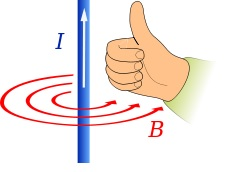
\includegraphics{images/chapter8/right_hand_rule.jpeg}
    \caption{Right hand rule} \label{c8_right_hand_rule:fig}
\end{figure}

Current (I) flowing through a wire and the change in the current generates EM
wave, so if we put an antenna next to the wire we will be able to pick up the
current on this wire next to the antenna and to do this we only need to get
close (do not need to cut anything open), which makes it more reasonable attack
model. The disadvantage is that we have much noise going on, and we will
have a lot of RF signal processing to do so it is not trivial to get from there
to the key. Let us assume we are doing PA without EM. So, our output now is a
data structure. This data structure has plain text, ciphertext, and power
consumption, but power consumption is not a fixed value, it is a trace vector.
Now, if we think about the device under test (DUT), most of the time, when we are
performing a measurement of the power consumption, it is not handling the
secret, it is doing something else. So if we look at the first byte of the key of
AES, it is processed at the beginning of the encryption where there is adding the
critical operation. The idea of AES is that every bit of the key will be mixed into
the whole ciphertext, so it is not easy to track it. At the beginning of
the encryption, the key is not being processed at all, and in the end, its affected
so dilute into the ciphertext. So there is going to be a particular time when
this trace is interesting. There
are only a few interesting points for an attacker from a very long trace with millions of points. In DPA, we had one number, the
time, and we knew that the signal was decoded in this number. We have a significant
vector, and we know the signal is somewhere in there, but it is not in all of the
points. However, we did the same thing here, we guessed a little part of the key, and then
we gave each one of the rows in the data structure a bit, one or zero. So, we
looked at some intermediate value, we have the AES state, and we took a
little bit of the state, and we gave each one of the rows in the data structure
again, a one-bit value and the one-bit value was precisely the value of this bit
of the state. We have a way of splitting our group of traces into two,
the same thing as the timing attack. We claim that if we guessed the bit correctly,
we just made a meaningful split of the traces. Now we divide our traces into two
sets, and we want to test if there are different distributions. We hope that at
some point (the correct time), there will be a proper distribution. An important
thing to understand is how many ways we have to split the traces into two in the
timing attack. If we guess one bit of the key, there are two ways of splitting.
Each time we decided we guessed a crucial bit, we simulate it a bit, and then
we gave each entry in the data structure value of 1 or 0. However, AES is a
byte-oriented algorithm, so there are 256 ways of splitting, i.e., We have 256
different competing ways of splitting the traces into two. However, again, we split
the traces into two. So, once we decide on a split, we go over the data structure, and each row, we assign a value of 1 or 0. Then we perform difference of means,
i.e., we take the mean of the right, the mean of the left, and 256
different ways of splitting into two and look at the difference of mean where we
get the most significant difference between the two means.

\section{Correlation Power Analysis (CPA)}\label{c8_cpa:sec}

\subsection{Hamming weight}\label{c8_CPA_hamming_weight:subsec}

The hamming weight \cite{hamming} of a number is the number of bits, which are set to 1 in its binary
representation. Hamming weight can refer to a hamming weight of the state, or to
hamming distance, which means how many bits change from one state to the
next. Let us assume we are looking at the hamming weight of a byte. This hamming
weight has values varying between 0 and 8. A number with hamming weight 0 will be 0, and
a number with hamming weight one will be a power of 2. For $m$ independent and uniformly
distributed bits, the whole word has an average Hamming weight $\mu_h = m/2$.

\subsection{CPA background}\label{c8_CPA_background:subsec}

We need to find a way to know when the traces are different. In DPA \cite{kocher1999differential, kocher1998introduction} we guessed
one byte of the key so we have 256 ways of splitting, but still, based on this
guess we only guess one bit of side-channel. So now we have 256 different ways
of splitting the ciphertext into two groups and if we guessed right, the two
groups will be different, but only at the correct time.
At previous lessons, we learned that most computers these days are based on
a technology called CMOS. CMOS's idea is that if nothing much is happening
if it is in a static state,  the power consumption is shallow. However, if it is
dynamic, if it switches between 1 and 0, there are bursts of power consumption.
So, in a CMOS device, the power instantaneous power consumption is correlated
with the number of bits that are flipping in this period. This fact was
completely ignored when we did DPA. We just said the power consumption was
different. As opposed to DPA, CPA does not ignore that fact. 

In CPA \cite{brier2004correlation, coron1962statistics, mayer2000smartly, oswald2003side},
we are going to guess one byte of the key, but we are not going to look
at one bit of the state. Instead, we are going to look at the hamming weight of the
state. Assume that if we guessed a byte correctly, the CPU is going to have to
handle a byte with it is the hamming weight. For example, if we guessed that the
state was 3, then the CPU will have to handle a byte with a hamming weight of 2.
Our data structure is plain text, and instead of a division to 0 or 1, we will
have a number between 0 and 8. This number is the hamming weight of the byte we
expecting the device to handle. Instead of splitting the traces into two groups,
we are going to use correlation. Due to CMOS, we can add a very reasonable claim
that when more bits are changing, the power consumption rises.

\subsection{CPA on AES motivation}

AES \cite{anderson1998serpent} is byte-oriented, so we have 256 different guesses. Now, we are trying to
give a label to each one of the inputs. We start with a guess, and then we give it
a label. The first step of AES is to take the bytes of the plain text and XOR
them with the secret key (bit-wise operation). The next step is to apply the sub-byte
transformation, which is a look-up table. After applying the sub-byte, we
have a byte, which is a mixture of the plain text that we know and the secret key. So if we guess a key, we can completely simulate the value. After
sub-byte, we apply shift-rows. However, shift-rows is just reading and writing the same
value from memory. It is reading this value (HW(S[P xor K])) and makes it
even stronger. Next, there is Mix columns operation. The mixColumns operation
uses 32 bits, so we will have $2^{32}$ different guesses to do mixColumns. Since $2^{32}$
is large number we will need many traces, and we will need to measure the DUT many times. Then we classify the measurements. There is going to be a statistically
meaningful classification for correct guesses. We refer readers to \cite{AESDescription} 
for a further detailed explanation of the AES algorithm.

\begin{figure}[!ht]
    \centering
    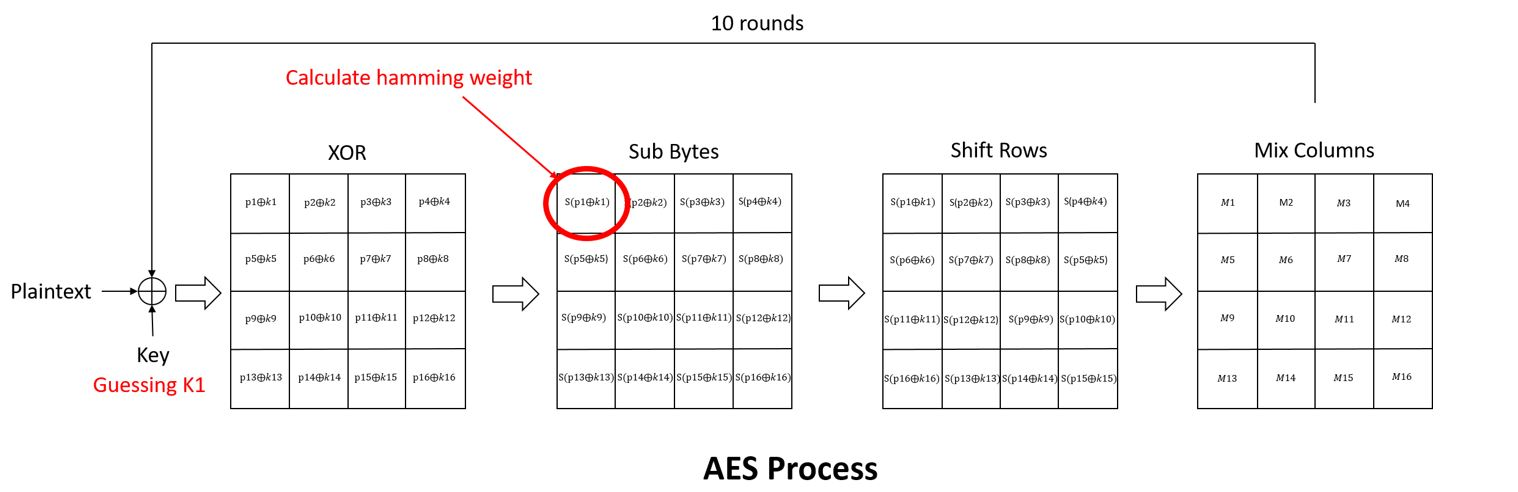
\includegraphics[width=1.0\textwidth]{images/chapter8/aes_process.jpg}
    \caption{AES illustration} \label{c8_aes:fig}
\end{figure}

In the timing attack days, we achieved a meaningful conclusion by running the students t-test
Moreover, getting a division into two setss and in DPA, we applied difference of means. To find
meaningful classification in CPA, we will need the statistical Pearson
Correlation Coefficient~\cite{PearsonCorrelationCoefficient}. The Correlation
Coefficient is simply the covariance normalized to a value between -1 and 1. The
intuition is that if the correlation coefficient is zero, it means we are
not guessing the key correctly, and if we are guessing the key correctly, we are
getting a correlation coefficient, which has a high value, notably better than what we get
on the other key guesses. 

\subsection{CPA's data structures}\label{c8_CPA_data_structures:subsec}

When we were looking at a timing attack, we had a data structure of size D; we
had D inputs; each input was a message we are trying to sign. For each of these
inputs, we had a trace, our side-channel trace which was a single number.
Our data structure was D times one. When we perform High Data Complexity power
analysis, we are going to do D different inputs, and each one of these lines
represents a single trace, i.e., long vector, and not a single point like the
timing attack. The vector with size T represents the power consumption of the device
running with the input in T different points of time. So we have a matrix data
structure of size D times T. D different inputs and T different times. Each line
of the matrix can be thought of as if we fix the plain text and ask the power
consumption over time of this plain text.

Each column of the matrix can be thought of as if we fix the time and ask what is the
power consumption of the device in that particular time. One of these times
called the correct time, and we will get the statistical meaning at that time. In
other incorrect times, we won't get any statistical meaning because the DUT is
not processing the data we are looking at.

Note that in order for the CPA attack to succeed, we have to align the traces to
the same time. Together with this matrix, we have another data structure, which contains
the inputs, so each one of these lines says, "this is the encryption of plain
text A, this is the encryption of plain text B," and so on. There are all sorts of
ways of getting it, depending on the attack model. One way is that the attacker
has a signing oracle, and the attacker chooses the plain texts and sends them to
the device. This is the most straightforward model of the attack. Another way which is a
little more confusing is that the attacker has to commit ahead of time all the
plain texts, and then the device encrypts them all at once, so he can't adapt to
whatever input he gives.

\subsection{CPA on AES step by step}\label{c8_CPA_overview:subsec}

We want to do a CPA on the AES encryption. We want to guess one byte of the key, and we want to get this byte mixed with the plain text, which we know. In addition, we
do not want too many bits of the key to getting mixed in because then we will have many guesses. So, the plain text comes in here, and we know the plain text. We
mix it with the unknown key. The key is a guess. How many guesses are there for
the key?  $2^{128}$ ways of guessing the key. However, to not guess the
entire key at once, we can guess only one byte at a time, so there are acually
256 guesses at each time. 

For a critical guess, We can simulate the key bit XOR plain text. Then, we can
simulate sub-byte of (key XOR plain text), and then we can also simulate
shift-rows on that result. This is where our simulation stops, because to
simulate mix-columns we need to guess 32 bits of the key, and we do not want to
guess 32 bits. The trick is that when the DUT is manipulating this value (the
the value we got after the simulation stopped), it will have some power consumption,
and that power consumption will be correlated to the hamming weight of that
value (according to the assumption we have on the CPA attack). 

Example: Let us assume we guessed the key byte as 5. So, if we know the guess of
the key byte is five, we can look at the plain text, and we know the first byte of
the plain text so that we can do key XOR plain text. We can do subByte of key XOR
plain text, and we can calculate the hamming weight of it. So, we have a vector
of size D, which is the hamming weight that we guessed for each one of the
inputs. We have a function that receives as the plain text and our guess as its input
and outputs the hamming weight. We have D different inputs, so we will call this
function D times and get an output of vector of size D. 

If we guessed the key correctly, at some point in time, which is called the
correct time, the power consumption would indeed be correlated (close to +-1)
with this vector that we guessed and all of the other times will not be
correlated (since the DUT is not only processing this byte of the key, but it is
processing other bytes of the key, other things, and more). However, at the correct
time, there is going to be a correlation. If we did not guess the right key,
there would be no time, which will correlate, meaning the correlation is
close to zero. If I say that there is a correlation, meaning the correlation is
close to +-1. 

\subsection{CPA warm up example}\label{c8_CPA_warm_up_example:subsec}

We have a DUT, we have a matrix of traces, we know the plain text, we know the
ciphertext, we know the power traces, and we know the key. So we have the power
trace, and we want to find where exactly inside the power trace is this bit being
processed. Our objective now is to find out when the DUT is processing the first
byte of the key. It could be interesting for us if we want to perform a fault attack \cite{FaultAttack}
Alternatively, a template attack \cite{TemplateAttack} or if we want to make sure that we know how to do CPA.
As we saw earlier, the hamming weight of the sub-byte output is a good
hypothesis.

Now, let us look at our data structure. We have a matrix of traces, D time T.
Lets assume we have 1000 traces. Each one of these traces covers an extended period, several milliseconds, so it has 1 million points. Each one of these values
is not Boolean. Usually, it is one byte if we are using a regular source code. We
also have the inputs; we know for each of these traces what was the plain
text being processed. The size of the plain text in AES is 16 bytes (128 bits).
So we have another data structure, which is 128 bit by 1000 rows, so each input
is 128 bit and has 1 Megabyte of a trace attached to it. We also know the key, so we
do not have to guess it. So now, we are trying to find out what is the correct
time. We want to find out, for example, when is the DUT processing the first byte
of the key. So we go over each one of our plain texts. We can do plain text XOR
key, we can also do sub-byte of that, and we can calculate the hamming weight of the output
of sub-byte. To each of the input plain texts, we associate the output hamming
weight. We hypothesize that the hamming weight the device will have to
manipulate is the output hamming weight we calculated. We created 1000 such
numbers. Each of the rows will now have plain text, trace, and hypothesis.

\begin{figure}[!ht]
    \centering
    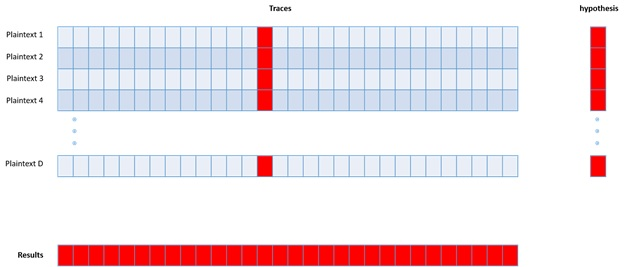
\includegraphics[width=1.0\textwidth]{images/chapter8/cpa_warmup_example.jpg}
    \caption{Graphic way of CPA warm up example} \label{c8_cpa_warmup_example:fig}
\end{figure}

The next step is to take the hypothesis and to sweep it across all moments. Assume we have a fixed specific moment in time, i.e., a vector of size 1
time 1000. This vector is the instantaneous power consumption of the device at
a fixed particular time. Recall that the hypothesis is also a vector of size 1
time 1000. For two vectors of size 1000, we calculate the Pearson Correlation
Coefficient. The Pearson Correlation Coefficient function receives as an input 2
vectors of 1 by 1000 and outputs a single value between -1 and 1. If this value
is very high or low, it means that there is a correlation between the input
vectors, but if it is close to zero, it means there is no correlation between the
vectors. We will execute this process for each fixed moment in time; in our
example, we will run in 1 million times. So the output of this step is a vector
of size of 1 million by 1. So 1 million different times, for each of these
times, we have a single value between -1 and 1. Now we can look at this and see
where the maximum absolute valued point is, and it is probably the correct time.

\subsection{CPA example}\label{c8_CPA_example:subsec}

However, in the warm-up example, we had one assumption that not always correct -
we assumed we know the key. In the following example, we want to do CPA in case
we do not know the key. We still have a matrix of traces. To each trace, we have
the associated input plain text. In order to solve the critical problem, we will run
the warm-up CPA 256 times. Each time we guess the key. If we are guessing the
key as 0, we will have a hypothesis vector, and we can sweep it and get a vector
of a million times one. We can also try a key one and sweep it again and get another
vector. For key 2, key three are all going to key 0xff, i.e., 256 different key
guesses, which gives us 256 times a million possible correlations. In this case,
we have 256 guesses and not a single hypothesis vector but a hypothesis matrix.
256 different hypotheses each column in the hypothesizes matrix is like the
warm-up. Then we take this matrix and sweep it across this matrix. In the end, we
get a million different time by 256 different key guesses, and each one of the
points in this matrix represents the correlation between our hypothesis and the
instantaneous power consumption of all of the devices at one particular moment
in time. So this is a two-dimensional matrix, and each row corresponds to a key, and each column corresponds to a time. So, most of the time, 99.9\%, this
matrix is going to be more or less 0. However, there are going to be some points where
there is a good correlation, and this point is at the correct time and the
correct key!

Let us do this in pictures. So, when we had a single hypothesis, we would take
this red row and sweep it across this red line, this was the warm-up. However, now
we do not know the key if it is red or blue or green, so we take this blue vector
and sweep it across, and we will take this green vector and sweep it across. So
this is the output here, it has the same number of rows as the number of key
guesses and the same number of columns as we have times. This is full CPA, and
hopefully, in one of these rows, we will have a peak, and we will be happy. 

\begin{figure}[!ht]
    \centering
    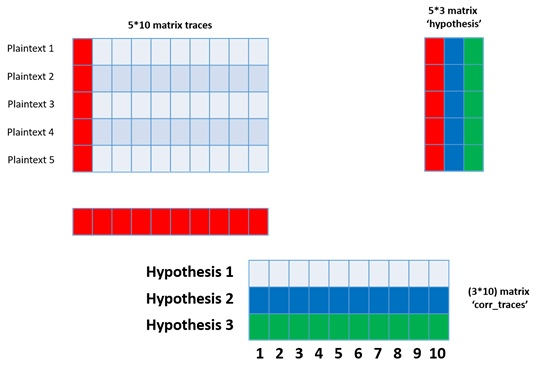
\includegraphics[width=1.0\textwidth]{images/chapter8/cpa_example.jpg}
    \caption{Graphic way of full CPA example} \label{c8_cpa_example:fig}
\end{figure}

\subsection{CPA in Matlab examples}\label{c6_Matlab_CPA_example:subsec}

We will show a Matlab example, which includes CPA, warm-up CPA, and the full CPA, as
seen in this section. We are working on a data set called WS2 \cite{WS2}, which is part of
the DPA toolkit. It has 200 traces, each one of size 30,000. These are power
traces of the first round of AES on an 8-bit microcontroller, which is deficient
in clock speed and is very vulnerable to DPA. Also, that test setup is a
lab setup, so this is the best we can hope for in terms of DPA. For each one of
the traces, the plain text is known. \Cref{fig:c8_Matlab_power_as_sample_number}
describes the 200 traces of power consumption as a function of the sample number. 

\begin{figure}[!ht]
    \centering
    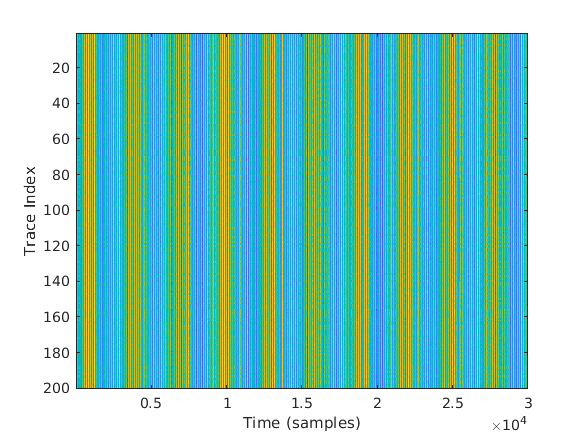
\includegraphics[width=1.0\textwidth]{images/chapter8/DataSet.png}
    \caption{Power consumption as a function of sample number} \label{fig:c8_Matlab_power_as_sample_number}
\end{figure}

The density of the colors indicates the instantaneous power consumption at a
particular moment at the DUT. The traces are very well aligned. Aligning is not
a simple task, but this device was aligned. It was a lab setup, so it is
easy to align. We can see that the device is doing the same thing at the same
time for all of these devices. If we zoom in, we will see a variation between
the traces. If we zoom in to two different traces, we will get figure
\ref{c8_Matlab_zoomin_on_two_traces:fig}.

\begin{figure}[!ht]
    \centering
    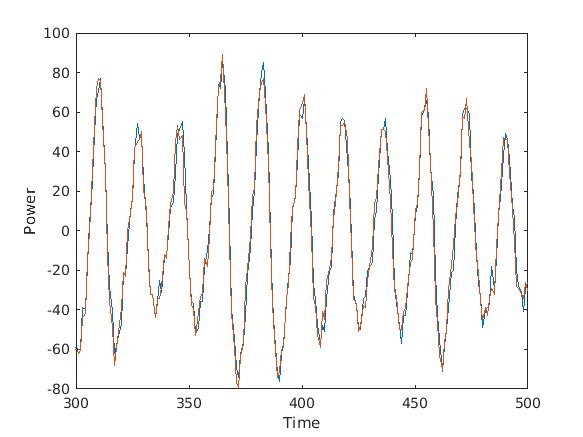
\includegraphics[width=1.0\textwidth]{images/chapter8/TwoSamples.png}
    \caption{Zoom-in on two different traces} \label{c8_Matlab_zoomin_on_two_traces:fig}
\end{figure}

The X-axis represents the time (in samples), and the Y-axis represents power.
The power consumption is between +-80. These two traces are very similar, but
there are some differences. The differences could be measurement noise or some
other signal processing.\\
For explanation, let us do the warm-up example. At this example, we know that the
first byte of the key is 120. Now that we know the key and the plain text, we
could say that when we are at the correct time, the DUT will be processing
a hamming weight of the correct key. In a DPA, first of all, we find the plain
text XOR the key, at first, we are looking only at the first byte, a result is
a number in the range of 0-255. Then we apply the AES subByte operation. Then we
are calculating the hamming weight of the outcome. The values of the results are
between 0 to 8. By doing this, we get the hypothesis\_vector for each particular
input.

\begin{figure}[!ht]
    \centering
    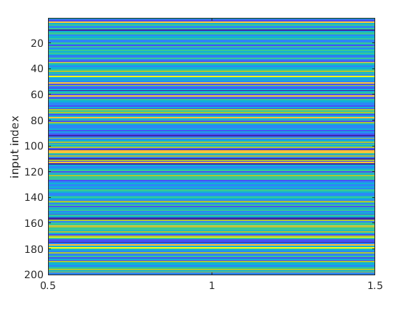
\includegraphics[width=1.0\textwidth]{images/chapter8/hypothesis_vector_values.png}
    \caption{Hypothesis vector values} \label{c8_Matlab_hypothesis_vector_values:fig}
\end{figure}


Figure \ref{c8_Matlab_hypothesis_vector_values:fig} presents the
hypothesis\_vector values (the X-axis is not important). For each trace (Y-axis)
we calculate the hamming distance (presented by different colors). Now that we
have figure \ref{fig:c8_Matlab_power_as_sample_number} and figure
\ref{c8_Matlab_hypothesis_vector_values:fig} we are going to sweep the later
figure over the former, and for  each time we are going to calculate the Pearson
Correlation Coefficient. Thus, for each position, we are going to get a number,
and this number will be between -1 and 1. Figure
\ref{c8_Matlab_pearson_correlation:fig} describes the results.

\begin{figure}[!ht]
    \centering
    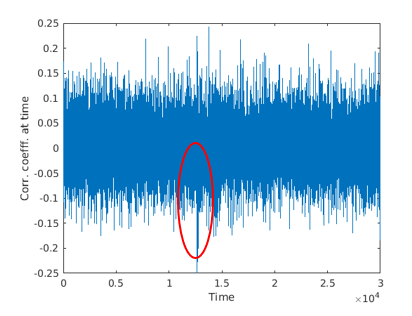
\includegraphics[width=1.0\textwidth]{images/chapter8/pearson_correlation_numbers.png}
    \caption{Pearson correlation graph} \label{c8_Matlab_pearson_correlation:fig}
\end{figure}

The X-axis is the time in samples, and the Y-axis is the Correlation Coefficient
between the hypothesis and the actual power consumption. Most of the time, it is
around +-1, but there is a peak described by the red circle. This peak describes
the time the AES is making the sub byte operation on the first byte of
the key. 

However, this was the warm-up example. In a real attack scenario, we do not know
the key. A real attack is very similar to the warm-up example, expect that we
are padding the key guessing by a loop and at this loop, we are checking all the
256 available for the key. A real attack is described at Figure
\ref{c8_Matlab_real_attack_scenario:fig}.

\begin{figure}[!ht]
    \centering
    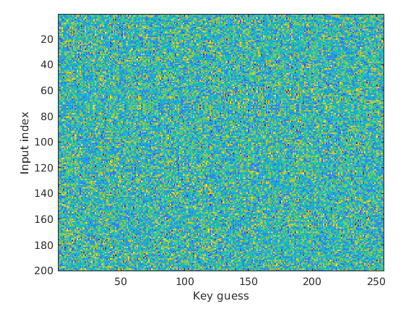
\includegraphics[width=1.0\textwidth]{images/chapter8/real_attack_scenario.png}
    \caption{Real attack scenario} \label{c8_Matlab_real_attack_scenario:fig}
\end{figure}

The X-axis is time, and the Y-axis is the key guesses. The color is the
correlation. Figure \ref{c8_Matlab_classification_matrix:fig} is the trace
classification matrix. The X-axis is time, and the Y-axis is the key guess. The
color is the correlation. From first glance, the correlation is more or less
0. However, there is on this matrix one high value. If we print out the
maximum of this matrix, we will get 0.9168, which is very far from zero.

\begin{figure}[!ht]
    \centering
    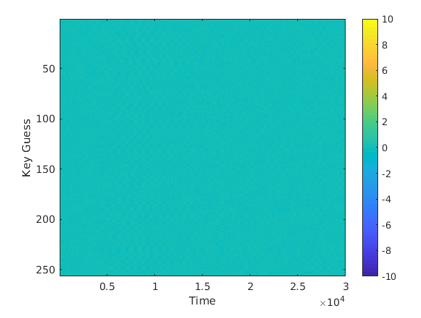
\includegraphics[width=1.0\textwidth]{images/chapter8/real_attack_classification_matrix.png}
    \caption{Real attack scenario classification matrix} \label{c8_Matlab_classification_matrix:fig}
\end{figure}

Now, we are going to find the correct time. The correct time is where there is a
maximum correlation, and the correct key is the row number of this value.  

\begin{figure}[!ht]
    \centering
    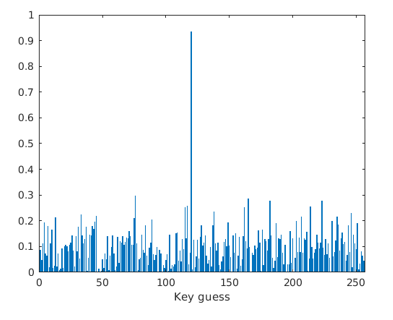
\includegraphics[width=1.0\textwidth]{images/chapter8/correct_time_graph.png}
    \caption{Correct time graph} \label{c8_Matlab_correct_time:fig}
\end{figure}

In Figure \ref{c8_Matlab_correct_time:fig} we are taking the classification
matrix shown in Figure \ref{c8_Matlab_classification_matrix:fig}  and we are looking at
the correct time. It has 256 different key guesses. The X-axis is the key guess, and the Y-axis is the correlation at the correct time. Most of the time, the
correlation is around 0.3, but at the correct key guess the correlation is 0.9.  

\begin{figure}[!ht]
    \centering
    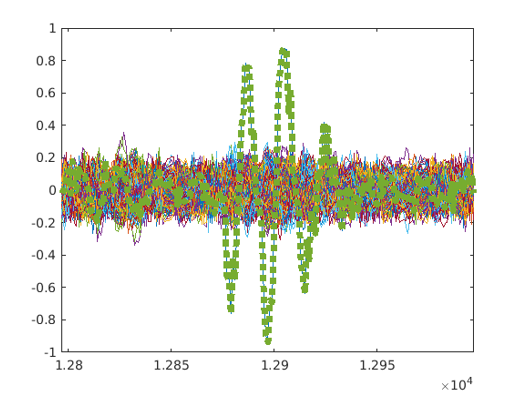
\includegraphics[width=1.0\textwidth]{images/chapter8/correlation_around_correct_time.png}
    \caption{Correlation around the correct time} \label{c8_Matlab_correlation_around_the_correct_time:fig}
\end{figure}

In Figure \ref{c8_Matlab_correlation_around_the_correct_time:fig} we can see the
correlation around the correct time. The green line is the correlation between the
correct key guesses, while the other lines indicate the wrong key
guesses at the correct time.

\begin{figure}[!ht]
    \centering
    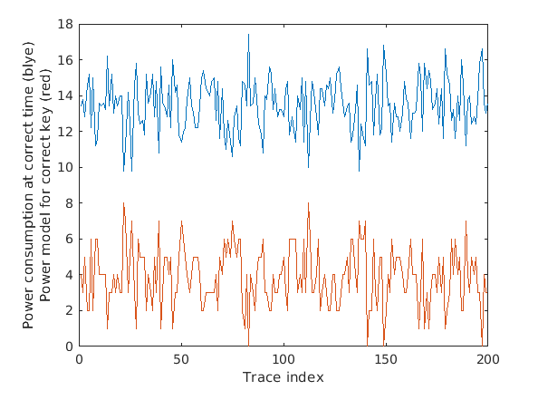
\includegraphics[width=1.0\textwidth]{images/chapter8/power_consumption_around_correct_time.png}
    \caption{Power consumption correlation around the correct time} \label{c8_Matlab_power_consumption_correlation_around_the_correct_time:fig}
\end{figure}

In addition, we can see in Figure
\ref{c8_Matlab_power_consumption_correlation_around_the_correct_time:fig} the
real power consumption of the DUT vs. the hypothesis. The blue line is the power
consumption of the DUT at the correct time. The Y-axis is traced. The red line
is the hypothesis that we tested. These two lines look correlated even to the naked
eye, and it is a negative correlation.

\subsection{Guest Lecture - Stjepan Picek}
We begin with an overview on the paper by Batina et al. \cite{batina2019csi}, which was presented at USENIX and co-authored by our guest lecturer.

\subsubsection{Introduction}
Machine learning has become quite mainstream in many industries of various domains, including security.
Organizations invest significantly in their artificial intelligence products, namely machine learning models which may even be the core intellectual property of a company.
The main research question of this study is the safety of machine learning applications and their susceptibility to physical attacks.
In this paper, the security of such models is studied from the point of view of a side-channel attacker, who seeks to reverse-engineer machine learning models and obtain information on it.
Using relatively simple side-channel analysis, it is shown that entire architectures of neural networks are leaked, including activation functions, number of layers and neurons, output classes and even weights.
Motivation for such attack can vary from wanting to build a surrogate model for an adversarial attack \cite{papernot2016transferability}, to privacy leakage of data in cases of sensitive medical or security applications.
Previous works investigated the leakage of sensitive information from machine learning models on individual data records or the entire training set.
More studies focused on reverse-engineering convolutional neural networks via timing and memory leakage, or exploiting line buffers in a convolution operation.
In this work, the focus is on commonly used neural network architectures, multilayer perceptron and convolutional neural networks, for their popularity and consisting of diverse types of layers.
Briefly, a neural network is composed of a number of layers, and each layer includes several neurons and parameters (weights), which process certain information and finally make a prediction according to some task.

\subsubsection{Threat Model}
The threat model in this paper includes the main goal of recovering the neural network architecture using only side-channel information.
There are no further assumptions on the data that is being processed, only that the target model does not include any side-channel countermeasures.
The attacker in consideration is passive, meaning she can only listen and acquire measurements of the normal operations of the device, without interfering at all.
No information on the model is assumed, but the attacker is able to query it using random inputs.
More capabilities include measuring side-channel information leaked from the implementation of the target architecture (Atmel ATmega328P and ARM Cortex-M3).

\subsubsection{Side-channel Analysis (SCA)}
DPA is a more advanced analysis, which uses statistical techniques to recover secret information from physical signatures.
The attack tests for statistically-significant dependencies between actual physical measurements (i.e., of power or electromagnetics) and hypothetical physical signatures (i.e., predictions on intermediate data).
The hypothetical signature is based on a leakage model and key hypothesis. A more detailed illustration can be found in Figure~\ref{fig:chapter8_dpa}.
The statistical analysis performed can be either difference of means or Pearson correlation, which will make it a differential analysis or correlation analysis, respectively.
The authors of this work used Pearson correlation, and therefore perform a correlation power analysis (CPA).

\begin{figure}
    \centering
    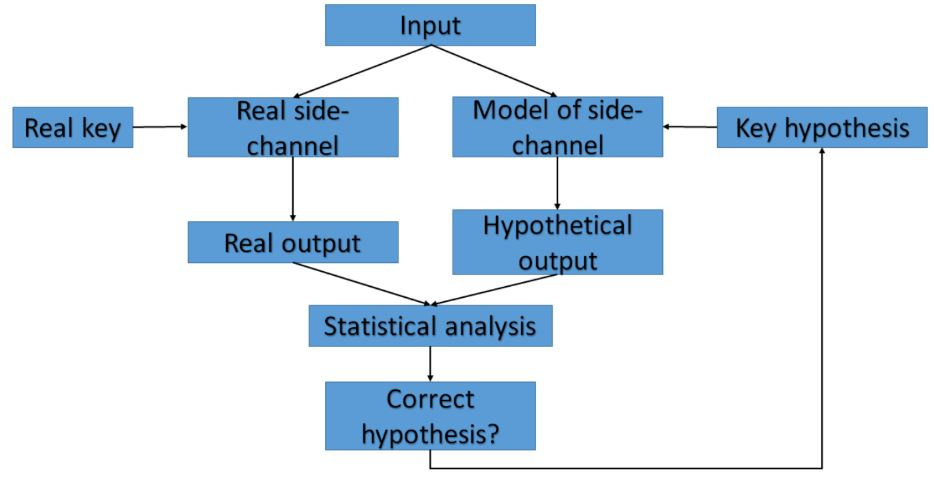
\includegraphics[width=0.9\textwidth]{images/chapter8/dpa.JPG}
    \caption{An illustration of the analysis process.}
    \label{fig:chapter8_dpa}
\end{figure}

\subsubsection{Experimental Setup}
The experiment was conducted using electromagnetics 
To gain a cleaner signal, the target microcontroller needed to be mechanically decapsulated, as shown in Figure~\ref{fig:chapter8_mc} along with the electromagnetic probe in Figure~\ref{fig:chapter8_probe} and the complete setup in Figure~\ref{fig:chapter8_complete}.
The exploited leakage model of the target device is the Hamming Weight (HW) model:
$$HW(x) = \sum{x_i}$$
A microcontroller loads sensitive data to a data bus in order to perform indicated instructions.
Note that the actual training phase is executed offline, and the final model is implemented in the C language and compiled on the microcontroller.
As discussed earlier, the goal is to obtain information on the neural network-based model, namely its layers, neurons, activation functions and weights.
The attack is therefore decomposed to four sub-goals, according to the type of target information.


\begin{figure}
    \centering
    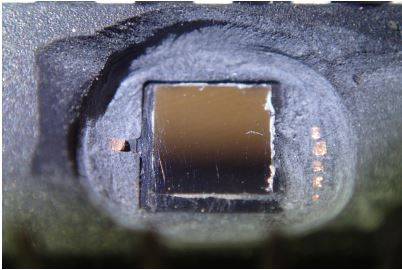
\includegraphics[width=0.9\textwidth]{images/chapter8/exp_a.JPG}
    \caption{8-bit microcontroller decomposed.}
    \label{fig:chapter8_mc}
\end{figure}

\begin{figure}
    \centering
    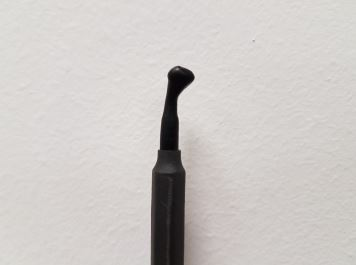
\includegraphics[width=0.9\textwidth]{images/chapter8/exp-b.JPG}
    \caption{Probe.}
    \label{fig:chapter8_probe}
\end{figure}

\begin{figure}
    \centering
    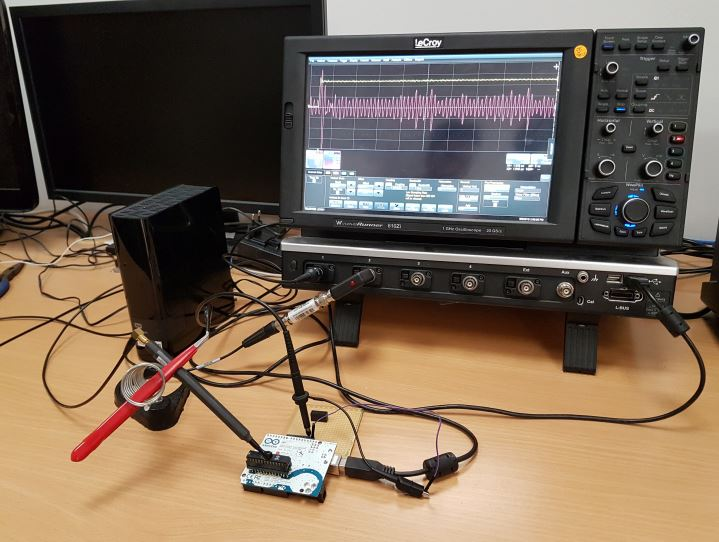
\includegraphics[width=0.9\textwidth]{images/chapter8/exp-c.JPG}
    \caption{Complete experimental setup and tools.}
    \label{fig:chapter8_complete}
\end{figure}

\subsubsection{Reverse-Engineering Activation Functions}
Recall that an activation function of some node is a function $f: \mathbb{R} \rightarrow \mathbb{R}$, as in:
$$f(x)=Activation(\sum(Weights * inputs) + bias)$$
There are many popular activation functions, with the most common ones being Sigmoid, Softmax, and ReLU.
The timing behavior of the various functions was observed directly on the electromagnetic (EM) trace, with a total of 2000 EM measurements captured.
By plotting the measurements, the difference in timings between the function can be easily observed (Figures~\ref{fig:activ-relu} \ref{fig:activ-sigmoid} \ref{fig:activ-tanh} \ref{fig:activ-softmax}), as well as statistically analyzed using maximum, minimum and mean values.

\begin{figure}
    \centering
    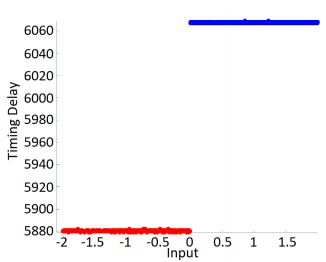
\includegraphics[width=0.5\textwidth]{images/chapter8/activ-relu-a.JPG}
    \caption{ReLU}
    \label{fig:activ-relu}
\end{figure}

\begin{figure}
    \centering
    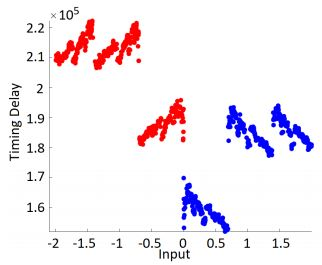
\includegraphics[width=0.5\textwidth]{images/chapter8/activ-sigmoid-b.JPG}
    \caption{Sigmoid}
    \label{fig:activ-sigmoid}
\end{figure}

\begin{figure}
    \centering
    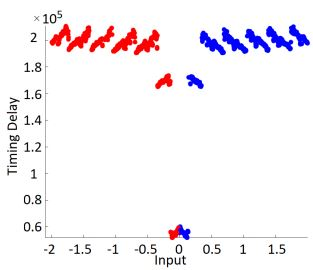
\includegraphics[width=0.5\textwidth]{images/chapter8/activ-tanh-c.JPG}
    \caption{tanh}
    \label{fig:activ-tanh}
\end{figure}

\begin{figure}
    \centering
    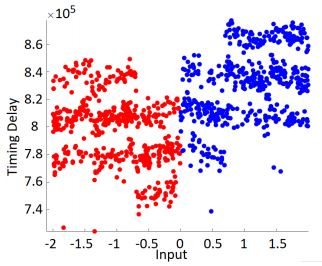
\includegraphics[width=0.5\textwidth]{images/chapter8/activ-softmax-d.JPG}
    \caption{Softmax}
    \label{fig:activ-softmax}
\end{figure}

\subsubsection{Reverse-Engineering Weights}
In this section, the CPA, i.e., Pearson correlation is used to extract parameters, or the weights of a layer.
CPA targets the multiplication operation $m=x*w$ where $x$ is a known input and $w$ a secret parameter.
Using the HW model, the adversary correlates the activity of the predicted output $m$ for all hypothesis of the weight.
Thus, the attack computes $p(t, w)$ for all hypothesis of the weight $w$, where $p$ is the Pearson correlation coefficient and $t$ is the side-channel measurement.
The correct value of the weight will result in a higher correlation, standing out from all other wrong hypothesis $w^*$, given we capture enough measurements.
We first need to understand the way the compiler is handling floating-point operations in our target device.
By analyzing the generated assembly, it can be confirmed that the device uses IEEE 754 compatible representation, with 32-bit consisting of: 1 sign bit, 8 biased exponent bits, and 23 mantissa bits, from $b_31$ to $b_0$ respectively.
The target device is an 8-bit microcontroller, so the 32-bit floating-point is stored in 4 registers.
Recall that we target the resulting multiplication of a known input and unknown weights, where for every input we assume different probabilities for weight values.
We then perform the multiplication accordingly and estimate the binary representation of the output, where the 23-bit mantissa is recovered first, and then the sign and exponent can be recovered separately.
Note that we need to recover the weight for every neuron separately, which may require a substantial amount of effort, while it is still feasible.

\subsubsection{Reverse-Engineering Layers and Neurons}
Simple observations of Figures~\ref{fig:layer-a},\ref{fig:layer-b},\ref{fig:layer-c} would show repeating patterns in each graph, which actually reveal the number of neurons.
As for the number of layers, or where the computation of each layer begins or ends (the red lines in the figures), we use CPA.
To determine if the targeted neuron is in the same layer as
previously attacked neurons, or in the next layer, we perform a weight recovery using two sets of data.
Let us assume that we are targeting the first hidden layer (the same approach can be done on different layers as well).
Assume that the input is a vector of length \(N_0\), so the input x can be represented x = \(x_1\),...,\(x_{N_0}\)
For the targeted neuron \(y_n\) in the hidden layer, perform the weight recovery on 2 different hypotheses.
For the first hypothesis, assume that the \(y_n\) is in the first hidden layer. Perform weight recovery individually using
\(x_i\), for \( 1\leq i \leq N_0\).
For the second hypothesis, assume that \(y_n\) is in the next
hidden layer (the second hidden layer).
Perform weight recovery individually using \(y_i\), for \(1\leq i \leq (n − i)\). For each hypothesis, record the maximum (absolute) correlation value, and compare both. Since the correlation depends on both inputs to the
multiplication operation, the incorrect hypothesis will result in a lower correlation value.

\begin{figure}
    \centering
    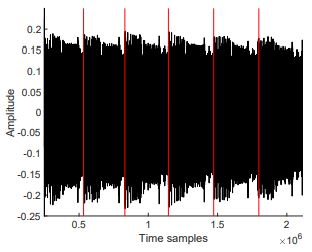
\includegraphics[width=0.5\textwidth]{images/chapter8/layer-a.JPG}
    \caption{One hidden layer with 6 neurons.}
    \label{fig:layer-a}
\end{figure}

\begin{figure}
    \centering
    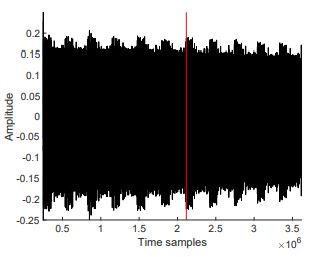
\includegraphics[width=0.5\textwidth]{images/chapter8/layer-b.JPG}
    \caption{Two hidden layers with 5 and 6 neurons respectively.}
    \label{fig:layer-b}
\end{figure}

\begin{figure}
    \centering
    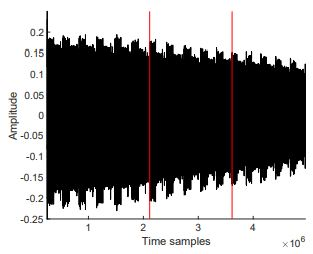
\includegraphics[width=0.5\textwidth]{images/chapter8/layer-c.JPG}
    \caption{Three hidden layers (6, 5, 5).}
    \label{fig:layer-c}
\end{figure}

\subsubsection{Recovery of the Full Network Layout}
The combination of previously developed individual techniques
can thereafter result in full reverse engineering of the network. The full network recovery is performed layer by layer, and for each layer, the weights for each neuron have to be recovered one at a time. The first step is to recover the weight \(w_{L_0}\) of each connection from the input layer \(L_0\) and the first hidden layer \(L_1\). In order to determine the output of the sum of the multiplications, the number of neurons in the layer must be known. Using the same set of traces, timing patterns for different inputs to the activation function can be built. The same steps are repeated in the subsequent layers \(L_1,...,L_{N-1}\)

\begin{figure}
    \centering
    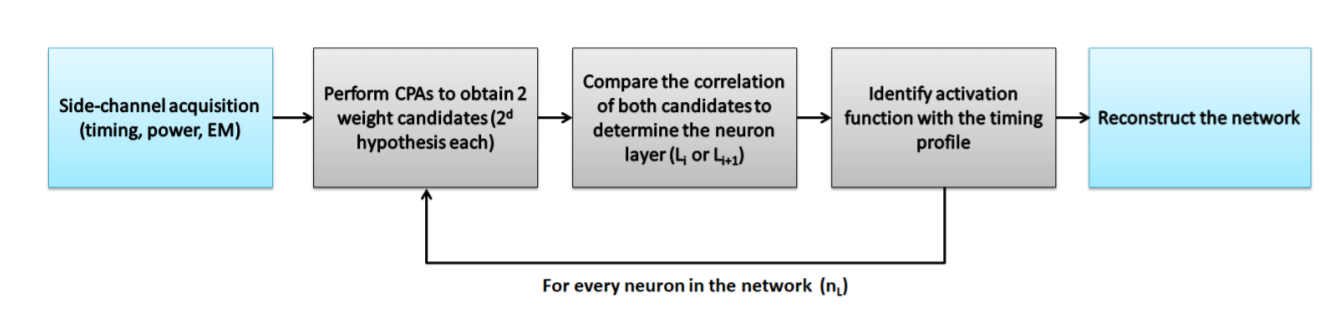
\includegraphics[width=100mm]{images/chapter8/reverse_methodology.PNG}
    \caption{Methodology to reverse engineer the target neural network}
\end{figure}

\subsubsection{Results}
In this experiment we used ARM Cortex M-3 processor. 
\newline
The first experiment done with MLP model and The databases MNIST and DPAv4.
For DPAv4 database the original accuracy equals 60.9\% and the accuracy of the reverse engineered network is 60.87\%.
For MNIST database the accuracy of the original network is equal to 98.16\% and the accuracy of the reverse engineered network equals 98.15\%, with an average weight error converging to 0.0025.
\newline
The second experiment done with CNN model and CIFAR-10 dataset. We choose as target the multiplication operation from the input with the weight, similar as in previous experiments. Differing from previous experiments, the operations on real values are here performed using fixed-point arithmetic. The numbers are stored using 8-bit data type – int8 (q7). The resulting multiplication is stored in temporary int variable. The original accuracy of the CNN equals 78.47\% and the
accuracy of the recovered CNN is 78.11\%.

\begin{figure}
    \centering
    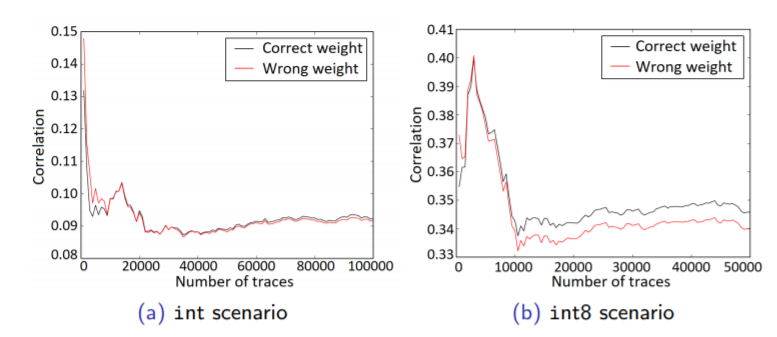
\includegraphics[scale=0.5]{images/chapter8/int_int8.PNG}
    \caption{The correlation of correct and wrong weight hypotheses on different number of
traces targeting the result of multiplication operation stored as different variable type:
(a) int, (b) int8}
\end{figure}

\subsubsection{Recovering the Input of Neural Networks}
The underlying neural network architecture of the used
network is public and all the weights are known.
Attacker is capable of measuring side-channel information
leaked from the implementation of the targeted architecture.
The crucial information for this work are the weights of the
first layer. Indeed, when MLP reads the input, it propagates it to all the nodes, performing basic arithmetic operations.
This arithmetic operation with different weights and common
unknown input leads to input recovery attack via side-channel.
The power consumption of loading data x is: 
$$HW(x) = \sum_{i=1}^{n} {x_i}$$
where \(x_i\) represents the \(i^{th}\) bit of x.
In our case, it is the product of secret input and known weight which is regularly stored to the memory after computation and results in the HW leakage.
\newline
The training phase is conducted offline, and the trained
network is then implemented in C language and compiled on
the microcontroller. In our experiments, we consider MLP architectures consisting of a different number of layers and nodes in those layers. Note, we are only interested in the input layer where a higher number of neurons is beneficial for the attacker. It can be extremely complex to recover the input by observing outputs from a known network. The proposed attack targets the multiplication operation in
the first hidden layer. The main target for CPA is the multiplication m = x · w of a known weight w with a secret input x. As x changes from one measurement (input) to another, information learned from one measurement cannot be used with another measurement, preventing any statistical analysis over a set of different inputs. 
\newline
To perform information exploitation over a single
measurement, we perform a horizontal attack. The weights in the first hidden layer are all multiplied with the
same input x, one after the other. M multiplications, corresponding to M different weights (or
neurons) in the first hidden layer are isolated.
A single trace is cut into M smaller traces, each one
corresponding to one multiplication with a known associated
weight. Next, the value of the input is statistically inferred by applying a standard CPA as explained before on the M smaller traces.

\begin{figure}
    \centering
    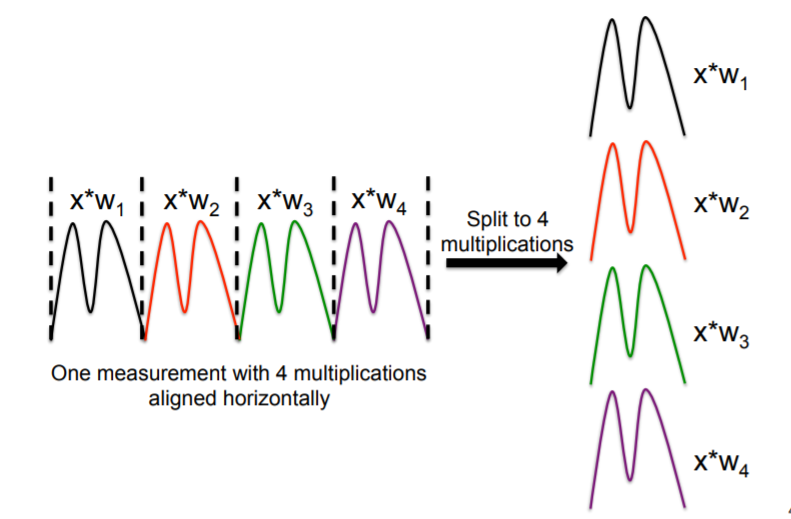
\includegraphics[scale=0.5]{images/chapter8/hpa.PNG}
   \caption{One measurement with 4 multiplications
aligned horizontally }
\end{figure}

\begin{figure}
    \centering
    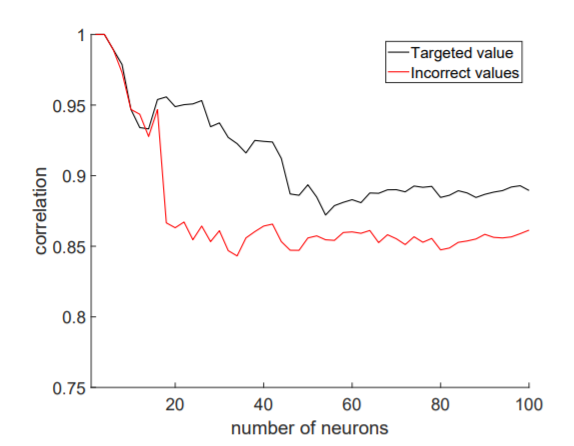
\includegraphics[scale=0.5]{images/chapter8/results.PNG}
    \caption{ Results on ATMega,
The first byte recovery (sign and 7-bit exponent).}
\end{figure}

The attack needs around 20 or more multiplications to reliably recover the input. In general, 70 multiplications are enough to recover all the bytes of the input, up to the desired precision of 2 decimal digits. This means that in the current setting, the proposed attack works very well on medium to large-sized networks, with at least 70 neurons in the first hidden layer, which is no issue in modern architectures used today.

\begin{figure}
    \centering
    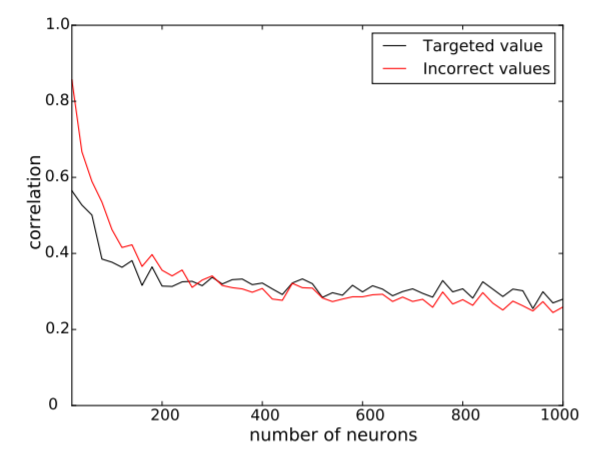
\includegraphics[scale=0.5]{images/chapter8/results2.PNG}
    \caption{ Results on ARM Cortex M3,
Correlation comparison between correct and incorrect inputs for target value
2.453.}
\end{figure}

\begin{figure}
    \centering
    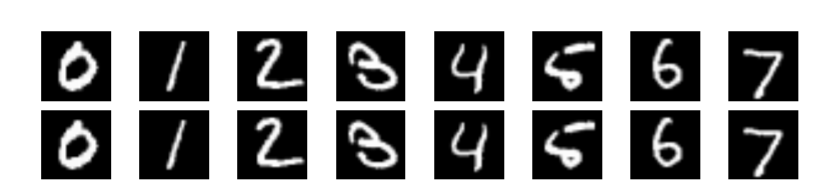
\includegraphics[scale=0.5]{images/chapter8/letters.PNG}
    \caption{ Attack on MNIST Database, Original images (top) and recovered images with precision error (bottom).}
\end{figure}

\subsubsection{Deep Learning and Side Channel Attacks}
Throughout history, many deep learning models have been built as described in Figure \ref{fig:deeplearning}.

\begin{figure}
    \centering
    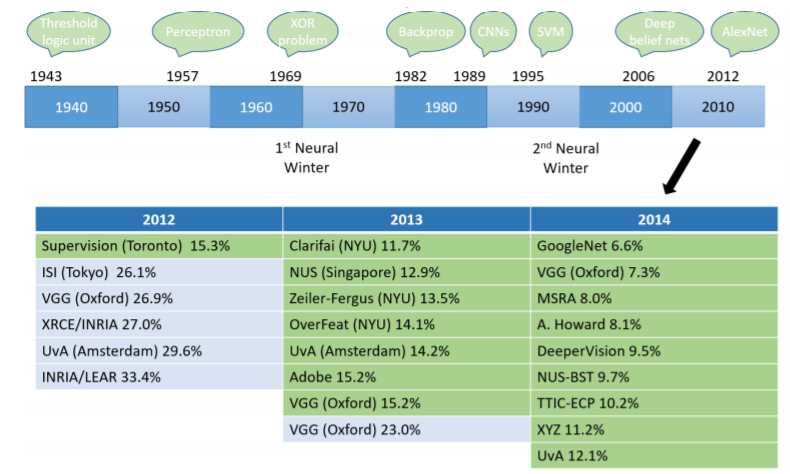
\includegraphics[scale=0.5]{images/chapter8/deeplearning.PNG}
    \caption{The history of the deep learning models}
    \label{fig:deeplearning}
\end{figure}

Deep learning is part of a broader family of machine learning methods based on artificial neural networks with representation learning. Learning can be supervised, semi-supervised or unsupervised.
\newline
A multilayer perceptron (MLP) is a class of feedforward artificial neural network (ANN). An MLP consists of at least three layers of nodes: an input layer, a hidden layer and an output layer. Except for the input nodes, each node is a neuron that uses a nonlinear activation function. MLP utilizes a supervised learning technique called backpropagation for training. Its multiple layers and non-linear activation distinguish MLP from a linear perceptron. It can distinguish data that is not linearly separable.

\begin{figure}
    \centering
    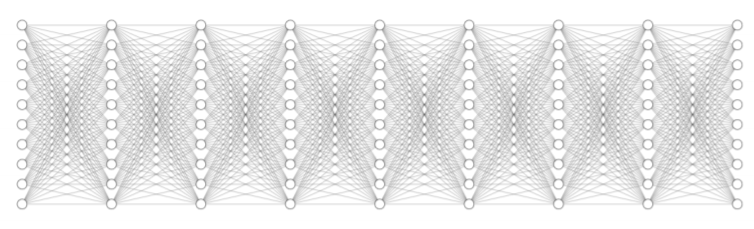
\includegraphics[scale=0.5]{images/chapter8/many_layers.PNG}
    \caption{Multilayer Perceptron - “Many” Hidden Layers}
\end{figure}

\begin{figure}
    \centering
    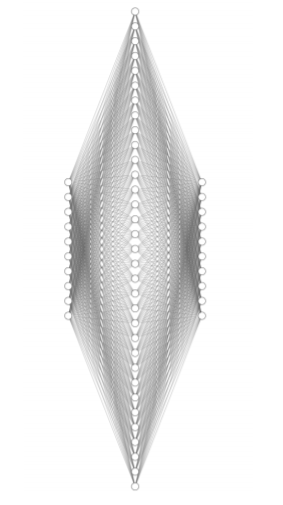
\includegraphics[scale=0.5]{images/chapter8/one_layer.PNG}
    \caption{Multilayer Perceptron - One Hidden Layers}
\end{figure}

The Universal Approximation Theorem states that a feed-forward network with a single hidden layer containing a
finite number of neurons can approximate continuous
functions on compact subsets of $\mathbb{R}_{^n}$. Given enough hidden units and enough data, multilayer perceptrons can approximate virtually any function to any desired accuracy. Valid results if and only if there is a sufficiently large number of training data in the series.
\newline
Convolutional Neural Networks represent a type of neural networks which were first designed for 2-dimensional convolutions. They are primarily used for image classification but lately, they have proven to be powerful classifiers in other domains. From the operational perspective, CNNs are similar to ordinary neural networks: they consist of a number of layers where each layer is made up of neurons. CNNs use three main types of layers: convolutional layers, pooling layers, and fully-connected layers as described in Figure \ref{fig:cna} .

\begin{figure}
    \centering
    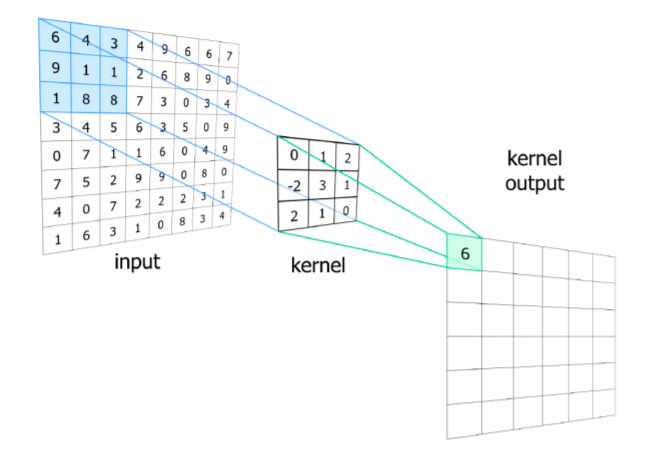
\includegraphics[scale=0.5]{images/chapter8/CNA.PNG}
    \caption{Convolutional Neural Networks - Convolution Layer}
    \label{fig:cna}
\end{figure}

The description of Convolutional Neural Network in SCA is described in Figure \ref{fig:cna_sca} .

\begin{figure}
    \centering
    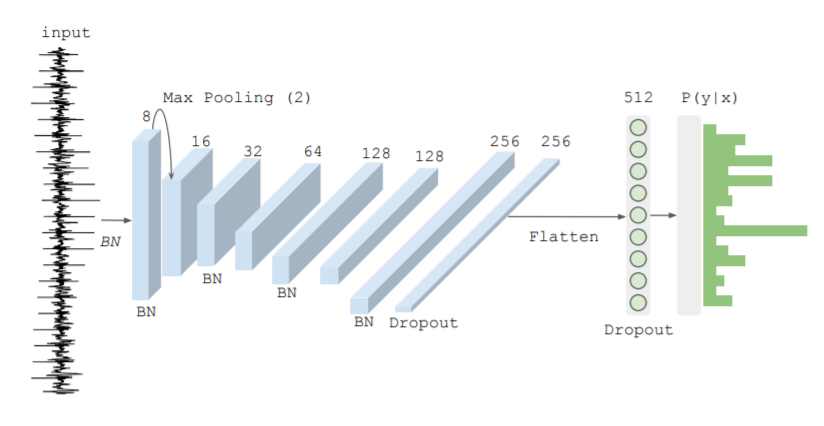
\includegraphics[scale=0.5]{images/chapter8/cnn_sca.PNG}
    \caption{Convolutional Neural Network in SCA}
    \label{fig:cna_sca}
\end{figure}

In our experiment we used 4 datasets as described in Figure \ref{fig:dbs_cna} .

\begin{figure}
    \centering
    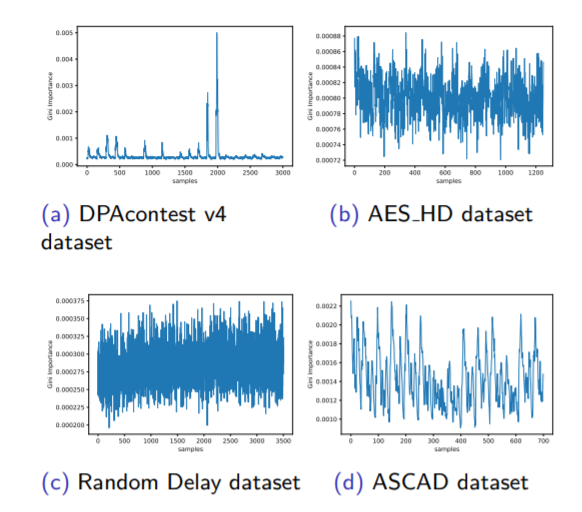
\includegraphics[scale=0.5]{images/chapter8/dbs_cna.PNG}
    \caption{Databases used for our experiment}
    \label{fig:dbs_cna}
\end{figure}

The results described in Figures \ref{fig:dpav4_results} \ref{fig:aes_rd_results} \ref{fig:ascad_results} .

\begin{figure}
    \centering
    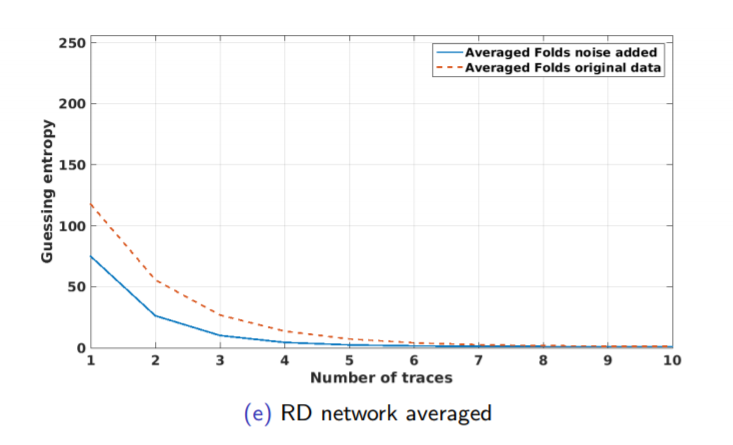
\includegraphics[scale=0.5]{images/chapter8/dpav4.PNG}
    \caption{Results for DPAv4 database}
    \label{fig:dpav4_results}
\end{figure}


\begin{figure}
    \centering
    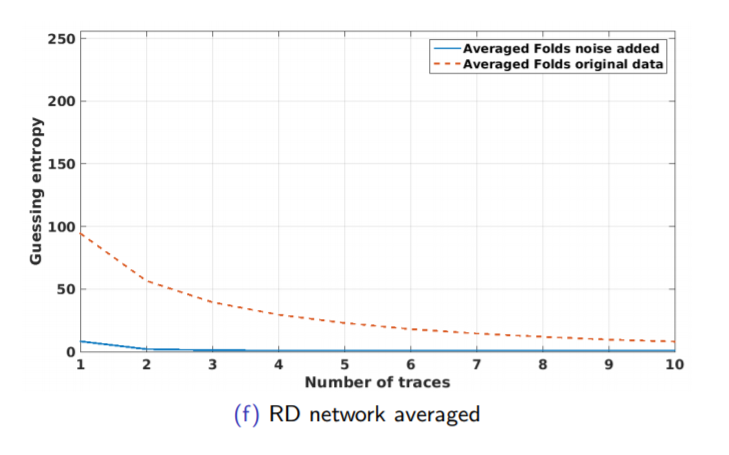
\includegraphics[scale=0.5]{images/chapter8/aes_rd.PNG}
    \caption{Results for AES\_RD database}
    \label{fig:aes_rd_results}
\end{figure}

\begin{figure}
    \centering
    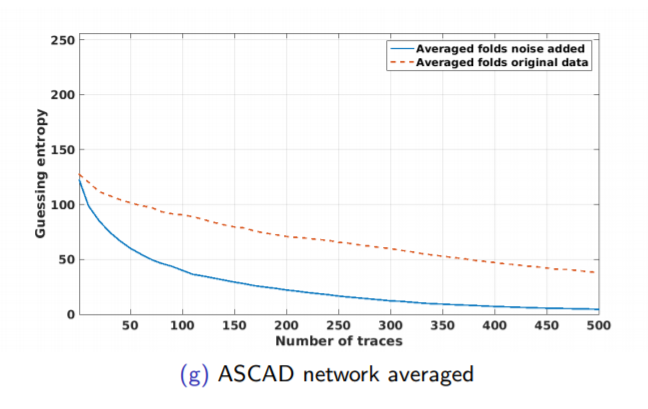
\includegraphics[scale=0.5]{images/chapter8/ascad.PNG}
    \caption{Results for ASCAD database}
    \label{fig:ascad_results}
\end{figure}

There are two devices: one for training and the second one for attack. Two devices means there are two different keys. Usually, we make our lives simpler and assume only one device and the same key, but this is not the same.
The setup for our experiment described in Figure \ref{fig:exp_setup} .

\begin{figure}
    \centering
    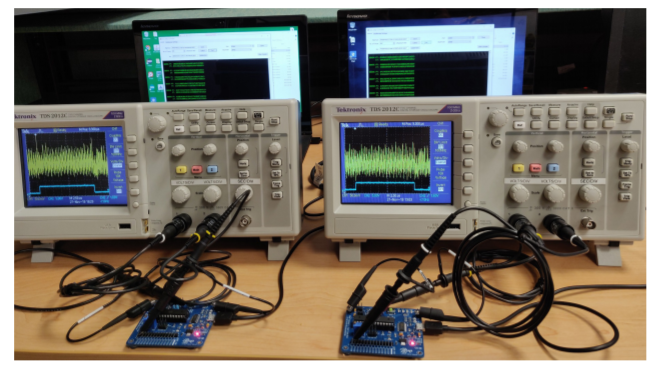
\includegraphics[scale=0.5]{images/chapter8/setup.PNG}
    \caption{Experiment setup}
    \label{fig:exp_setup}
\end{figure}

We tried multiple models. Same key and device as in \ref{fig:same_key_same_device} , Different key and same device as in \ref{fig:different_key_same_device} , same key and different device as in \ref{fig:same_key_differnet_device}, and different key and device as in \ref{fig:different_key_differnet_device} .The validation for our models describe in figure \ref{fig:validation} .

\begin{figure}
    \centering
    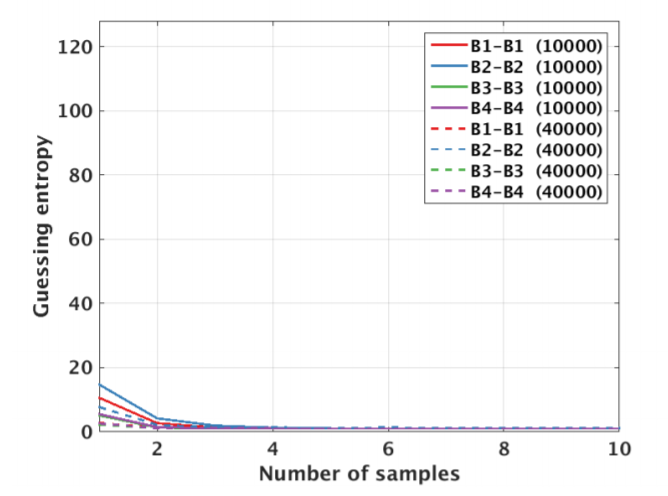
\includegraphics[scale=0.5]{images/chapter8/same_key_same_device.PNG}
    \caption{Same key same device results}
    \label{fig:same_key_same_device}
\end{figure}

\begin{figure}
    \centering
    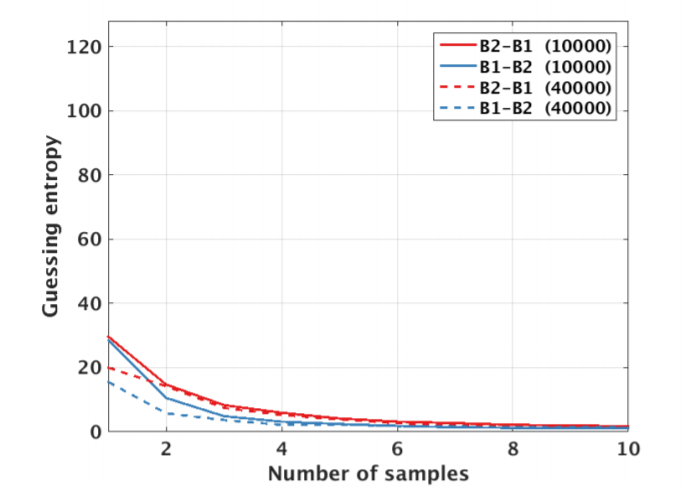
\includegraphics[scale=0.5]{images/chapter8/same_key_different_device.PNG}
    \caption{Same key different device results}
    \label{fig:same_key_differnet_device}
\end{figure}

\begin{figure}
    \centering
    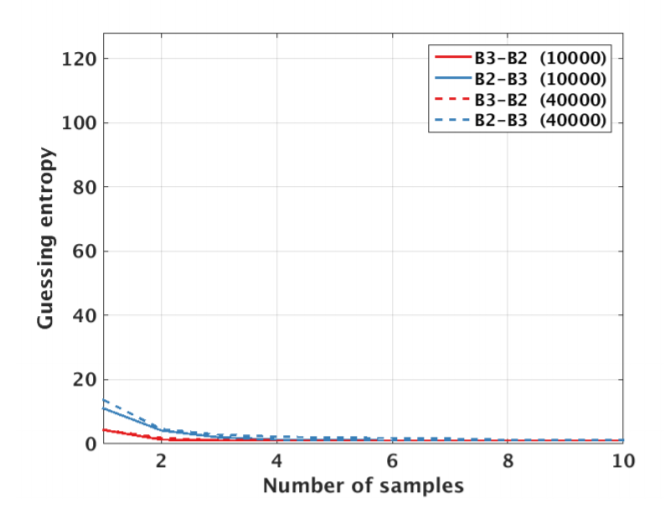
\includegraphics[scale=0.5]{images/chapter8/different_key_same_device.PNG}
    \caption{Different key same device results}
    \label{fig:different_key_same_device}
\end{figure}

\begin{figure}
    \centering
    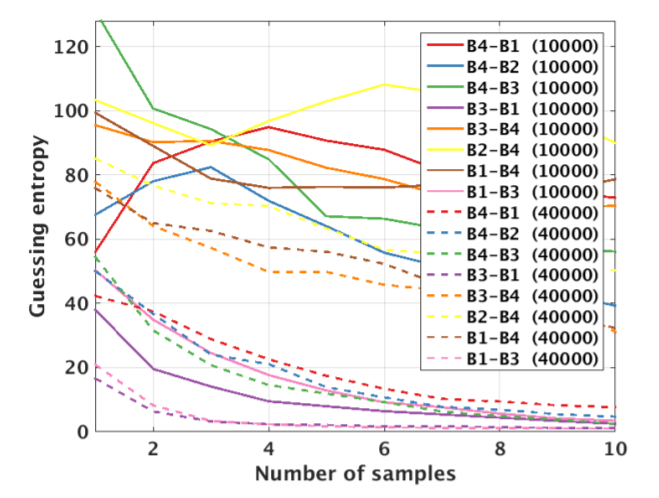
\includegraphics[scale=0.5]{images/chapter8/different_key_different_device.PNG}
    \caption{Different key different device results}
    \label{fig:different_key_differnet_device}
\end{figure}

\begin{figure}
    \centering
    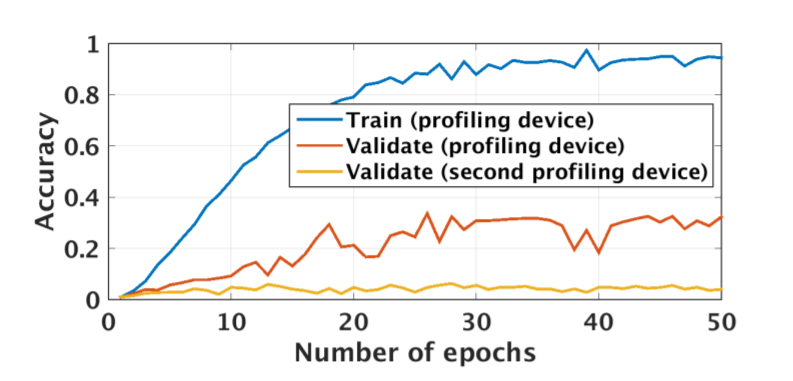
\includegraphics[scale=0.5]{images/chapter8/validation.PNG}
    \caption{Validation for our experiment}
    \label{fig:validation}
\end{figure}

Regarding multiple device model, instead of validating on the same device as training, we need
one more device. Separate devices for train, validation, attack. If we do not have a third device, we can use artificial noise. The multiple model describe in Figure \ref{fig:multidevice} .
 

\begin{figure}
    \centering
    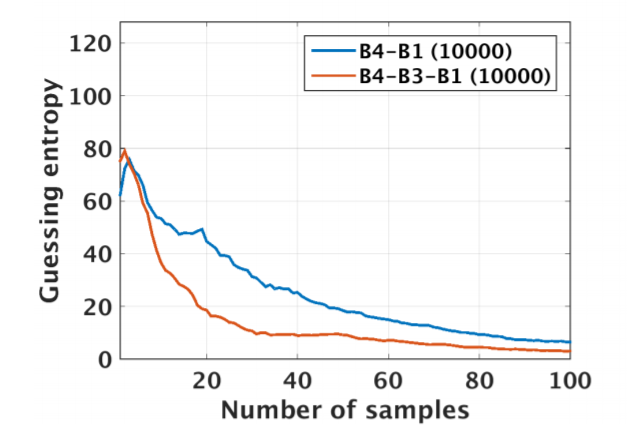
\includegraphics[scale=0.5]{images/chapter8/multidevice.PNG}
    \caption{Multidevice model results}
    \label{fig:multidevice}
\end{figure}
\subsection{Guest Lecture - Jiska Classen}
The thesis Jiska Classen supervised focused on finding errors in random number generators for bluetooth devices, as the bluetooth specifications just states that the random number generator needs to be secure but not specifies how.
In general, if some RNG does not pass statistical tests, it can be obviously broken.
But even if it does pass those tests it could still be broken.\\


\underline{The thesis focused on RNG variants 2 and 3:}
\begin{table}[htb]
\small
\caption{RNG variants 2 and 3}
\begin{adjustbox}{width=\textwidth}

\begin{tabular}{|l|l|l|l|l|l|}
\hline
\textbf{Device}  & \textbf{Chip Date} & \textbf{Variant} & \textbf{HRNG Location} & \textbf{Prng}                                                                       & \textbf{Cache}                  \\ \hline
Google   Nexus 5 & Dec 11   2012      & 2                & 0x314004,   3 regs     & Yes   (inline)                                                                      & No                              \\ \hline
MacBook   2016   & Oct 22   2015      & 2                & 0x314004,   3 regs     & Yes   (inline)                                                                      & No                              \\ \hline
CYW20735B1       & Jan 18   2018      & 3                & 0x352600,   3 regs     & \begin{tabular}[c]{@{}l@{}}Yes   (rgb\_ger\_psrng)\\    \\ 8 registers\end{tabular} & Yes,   breaks after 32 elements \\ \hline
CYW20819A1       & May 22   2018      & 3                & 0x352600,   3 regs     & \begin{tabular}[c]{@{}l@{}}Yes   (rgb\_ger\_psrng)\\    \\ 5 registers\end{tabular} & Yes (with   minor fixes)        \\ \hline
\end{tabular}
\end{adjustbox}

\end{table}

Using IDA, it was found that the HRNG (Hardware Random Number Generator) is mapped to a specific register, which is used to access it by the software (the address of this register varies between different chips). HRNG are mostly secure.\\
Different constants mark the state of the PRNG, one of them ("RBG\_CONST\_READY") is kind of a standard, so it can be also used to find the relevant disassembled code in a binary.
If the HRNG is not available, there is a RNG fallback, looking at the RNG Variant 2 implementation it was found that it is computed using the system and bluetooth clocks, frequencies and error streams, and uses not-random functions, as crc32.
Also, the input data is shown to not distribute equally. As a good thing, it does not use cache.

\begin{figure}[!ht]
    \centering
    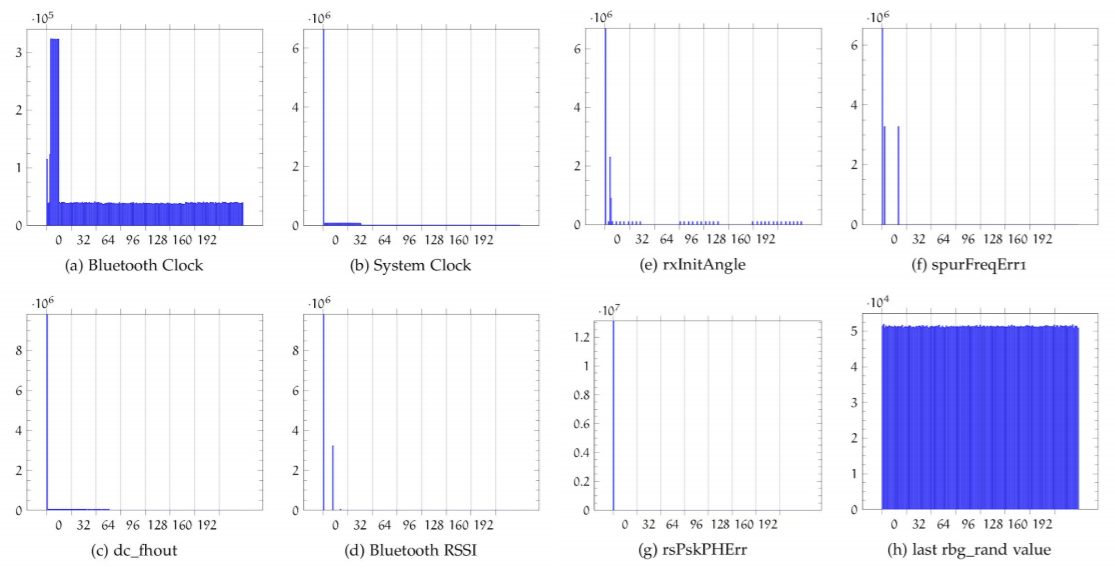
\includegraphics[width=\textwidth]{images/PRNG_Nexus5.png}
    \caption{PRNG measurements taken on a Google Nexus 5 (BCM4335C0)}
\end{figure}
\newpage
After finding that, CVE-2020-6616 was assigned to this discovery, which was later related by some companies, including Apple, in their fixes of the vulnerability.
Investigating 20 more devices and firmwares had trouble as some devices are slow(4 byte packages) and 1GB of data is needed to test the output quality of the random devices.


\begin{table}[htb]
    \caption{Chips challenged with Dieharder test}	
    \begin{adjustbox}{width=\textwidth}
        \begin{tabular}{|l|l|l|l|l}
            \cline{1-4}
            \textbf{Chip} & \textbf{Device}                      & \textbf{Samples} & \textbf{Dieharder} &  \\ \cline{1-4}
            BCM4335C0     & Google   Nexus 5                     & 2.7GB            & Passed             &  \\ \cline{1-4}
            BCM4358A3     & Samsung   Galaxy S6, Google Nexus 6P & 2.1GB            & Passed             &  \\ \cline{1-4}
            BCM43430A1    & Raspberry   Pi 3/Zero W              & 1.3GB            & Passed             &  \\ \cline{1-4}
            BCM4345C0     & Raspberry   Pi 3+/4                  & 1.4GB            & Passed             &  \\ \cline{1-4}
            BCM4345B0     & iPhone 6                             & 1.8GB            & Passed             &  \\ \cline{1-4}
            BCM4355C0     & iPhone 7                             & 1.0GB            & Passed             &  \\ \cline{1-4}
            CYW20719B1    & Evaluation   Board                   & 1.4GB            & Passed             &  \\ \cline{1-4}
            CYW20735B1    & Evaluation   Board                   & 1.6GB            & Passed             &  \\ \cline{1-4}
            CYW20819A1    & Evaluation   Board                   & 1.2GB            & Passed             &  \\ \cline{1-4}
            BCM2046A2     & iMac Late   2009                     & -                & HRNG               &  \\ \cline{1-4}
            BCM4375B1     & Samsung   Galaxy S10/S20             & -                & HRNG               &  \\ \cline{1-4}
            BCM4378B1     & iPhone 11                            & -                & HRNG               &  \\ \cline{1-4}
        \end{tabular}
    \end{adjustbox}
    \end{table}
    \break
    Many devices passed the Dieharder tests, for sample sizes of 1GB+, so they look ok.
    
    Other RNG variants, such as Variant 1, used by 2009 iMac or a 2010 Asus Dongle, which is the Fallback of the HRNG, used the basic rbg\_rand function which is only using the system clock and a static value and a register as an input for it’s PRNG, which is really bad.
    
    \begin{table}[htb]
                \caption{Variant 1}	
                \begin{adjustbox}{width=\textwidth}

        \begin{tabular}{llllll}
            \hline
            \multicolumn{1}{|l|}{\textbf{Device}}   & \multicolumn{1}{l|}{\textbf{Chip Date}} & \multicolumn{1}{l|}{\textbf{Variant}} & \multicolumn{1}{l|}{\textbf{HRNG Location}} & \multicolumn{1}{l|}{\textbf{PRNG}}      & \multicolumn{1}{l|}{\textbf{Cache}} \\ \hline
            \multicolumn{1}{|l|}{iMac Late   2009}  & \multicolumn{1}{l|}{2007}               & \multicolumn{1}{l|}{1}                & \multicolumn{1}{l|}{0xE9A00, 3   regs}      & \multicolumn{1}{l|}{Minimal   (inline)} & \multicolumn{1}{l|}{No}             \\ \hline
            \multicolumn{1}{|l|}{Asus USB   Dongle} & \multicolumn{1}{l|}{Feb 2010}           & \multicolumn{1}{l|}{1}                & \multicolumn{1}{l|}{0xEA204, 3   regs}      & \multicolumn{1}{l|}{Minimal   (inline)} & \multicolumn{1}{l|}{No}             \\ \hline
            &                                         &                                       &                                             &                                         &                                    
        \end{tabular}
    \end{adjustbox}

    \end{table}
    
    More investigation found that RNG Variants 2 and 3 is used by many more devices, from 2012 till 2018, and also being used by some ciphers chips:
    
    % Please add the following required packages to your document preamble:
    % \usepackage[normalem]{ulem}
    % \useunder{\uline}{\ul}{}
    \begin{table}[htb]
            \caption{Variant 2,3}	
            \begin{adjustbox}{width=\textwidth}

        \begin{tabular}{|l|l|l|l|l|l|}
            \hline
            \textbf{Device}                      & \textbf{Chip Date} & \textbf{Variant} & \textbf{HRNG Location} & \textbf{PRNG}                        & \textbf{Cache}                  \\ \hline
            Google   Nexus 5                     & Dec 11   2012      & 2                & 0x314004,   3 regs     & Yes   (inline)                       & No                              \\ \hline
            iPhone 6                             & Jul 15   2013      & 2                & 0x314004,   3 regs     & Yes   (inline)                       & No                              \\ \hline
            Raspberry   Pi 3/Zero W              & Jun 2 2014         & 2                & 0x352600,   3 regs     & Yes   (inline)                       & No                              \\ \hline
            Raspberry   Pi 3+/4                  & Aug 19   2014      & 2                & 0x314004,   3 regs     & Yes   (inline)                       & No                              \\ \hline
            Samsung   Galaxy S6, Google Nexus 6P & Oct 23   2014      & 2                & 0x314004,   3 regs     & Yes   (inline)                       & No                              \\ \hline
            iPhone SE                            & Jan 27   2015      & 2                & 0x314004,   3 regs     & Yes   (inline)                       & No                              \\ \hline
            iPhone 7                             & Sep 14   2015      & 2                & 0x352600,   3 regs     & Yes   (inline)                       & No                              \\ \hline
            MacBook   2016/2017, iMac 2017       & Oct 22   2015      & 2                & 0x314004,   3 regs     & Yes   (inline)                       & No                              \\ \hline
            CYW20719B1                           & Jan 17   2017      & 2                & 0x352600,   3 regs     & Yes   (inline)                       & No                              \\ \hline
            CYW20735B1                           & Jan 18   2018      & 3                & 0x352600,   3 regs     & Yes   (rbg\_get\_psrng), 8 registers & Yes,   breaks after 32 elements \\ \hline
            CYW20819A1                           & May 22   2018      & 3                & 0x352600,   3 regs     & Yes   (rbg\_get\_psrng), 5 registers & Yes (with   minor fixes)        \\ \hline
        \end{tabular}
    \end{adjustbox}

    \end{table}
    
    Variant 5 is used by much newer devices, iPhone 8 from 2016 till iPhone 11 and Samsung Galaxy S10 from 2018, where PRNG is gone and it has a cache for random numbers, which is a really bad idea.
    
    \begin{table}[htb]
                \caption{Variant 5}	
                \begin{adjustbox}{width=\textwidth}

        \begin{tabular}{|l|l|l|l|l|l|}
            \hline
            \textbf{Device}          & \textbf{Chip Date} & \textbf{Variant}                                                                                                               & \textbf{HRNG Location} & \textbf{PRNG} & \textbf{Cache}           \\ \hline
            iPhone   8/X/XR          & Oct 11   2016      & \begin{tabular}[c]{@{}l@{}}Variant \#3\\    \\ Complete   rework of rbg\_ library, but still using sha128 wrapper\end{tabular} & 0x352600,   4 regs     & None          & Asynchronous   32x cache \\ \hline
            Samsung   Galaxy S10/S20 & Apr 13   2018      & Variant \#3                                                                                                                    & 0x352600,   4 regs     & None          & Asynchronous   32x cache \\ \hline
            iPhone 11                & Oct 25   2018      & Variant \#3                                                                                                                    & 0x352600,   4 regs     & None          & Asynchronous   32x cache \\ \hline
        \end{tabular}
    \end{adjustbox}

    \end{table}
    
    \break
    Variant 4 has only PRNG, and was used by the Samsung Galaxy 8 since 2016.
    It uses the previous random string, hardware clock and some bitchanges, and even some constant values, all of these are bad habits for defining a PRNG.
    Inspecting Variant 4 inputs shows that they are not so random:
    
    
    \begin{table}[htb]
                    \caption{Variant 4 inputs}
                    \begin{adjustbox}{width=\textwidth}

        \begin{tabular}{|l|l|l|ll}
            \cline{1-3}
            \textbf{Address} & \textbf{Register} & \textbf{Entropy}                                                                               &  &  \\ \cline{1-3}
            -                & Rand              & Previous 4   B random value (leaks over-the-air)                                               &  &  \\ \cline{1-3}
            0x3180088        & dc\_nbtc\_clk     & Bluetooth  clock, publicly available over-the-air                                              &  &  \\ \cline{1-3}
            0x32A004         & timer1value       & Hardware   clock, 4 B "random" before first leak, unpatched  attacks for clock reset available &  &  \\ \cline{1-3}
            0x3186A0         & dc\_fhout         & Changes a   bit (0x02-0x50)                                                                    &  &  \\ \cline{1-3}
            0x410434         & agcStatus         & Changes a   bit (0xc00 during whole measurement, slight changes within 0xcnn after   reboot)   &  &  \\ \cline{1-3}
            0x41079C         & rxInitAngle       & Changes a   bit but within similar range                                                       &  &  \\ \cline{1-3}
            0X410548         & spurFreqErr1      & Constant   2B value (0x04ed, also after reboot)                                                &  &  \\ \cline{1-3}
            0x410548         & rxPskPhErr5       & Always 0                                                                                       &  &  \\ \cline{1-3}
        \end{tabular}
    \end{adjustbox}

    \end{table}
    
    In addition, looking at IDA’s disassembly, the random function is used by a lot of other functions, which are, in their turn, also used by many more functions.
    \\
    The effects of this work is that the new iOS mentioned those findings in it’s firmware release.
    The results were also sent to Qualcomm and broadcom, where they unveiled the clear results and effects.
    Separately, self controlled PRNG can be used to find out the random numbers used while connecting between 2 devices (Man in the middle).
    An ETA patch was sent on February and May 1.
    Broadcom didn’t give an ETA or any clarification about the found vulnerability or solution.
    
    The main conclusions are:
    \begin{itemize}
    \item Don’t trust embedded RNG.
    \item Collect a lot of data (+1GB) and verify the RNG quality.
    \item Each Broadcom firmware version has bugs.
    \end{itemize}
    The scripts used in this work can be found at \href{https://github.com/seemoo-lab/InternalBlue} github  
